\chapter{Mission Heritage}
\label{heritage}
\graphicspath{{chapter-1/Images/}}

%general introduction - opening paragraph
Asteroids and comets have been the target of many spacecraft missions in the past two decades, yielding unparalleled scientific returns relative to ground-based observations. Several space agencies, both private (such as Deep Space Industries and Planetary Resources) and governmental, are planning future missions to these small bodies to not only study them in more detail but also to manipulate, deflect and extract resources from them. The current chapter shall highlight past and current missions to small bodies in \Cref{past_current} and future missions in \Cref{future}.

\section{Past and Current Missions}
\label{past_current}
%talk about distant flybys as well as rendezvous missions here, both for asteroids and comets
A brief overview on missions to asteroids and comets that have flown in past or are still active at the time of writing this report will be presented in this section. The various missions will be presented in a reverse chronological order.

\subsection{Hayabusa 2}
\label{hayabusa2}
Hayabusa 2 is a \gls{JAXA} mission, launched on 3 December 2014. It will rendezvous with asteroid 1999 JU3 in 2018 and will return back to Earth with a sample from the asteroid in 2020. Hayabusa 2 carries an impactor that shall be used to create a crater on the asteroid to expose fresh material that will be collected and returned to Earth for further analysis \cite{hayabusa2}. Hayabusa 2 is a sequel to a previous asteroid mission by \gls{JAXA}, called Hayabusa which explored the asteroid Itokawa.

The asteroid 1999 JU3 (and henceforth JU3) has been classified as a potentially hazardous asteroid which also happens to be in the list of potential targets for another sample return mission: OSIRIS-REx of \gls{NASA} (briefed in \Cref{osiris-rex}). JU3 was also a potential target for the Marco Polo-R mission of \gls{ESA} as part of their Cosmic Vision Program, however in February 2014 it was not selected for the M3 Launch opportunity in the Cosmic Vision Program \cite{marcopolor}. JU3 has an orbit with semi-major axis of 1.19 \gls{AU} and an eccentricity of 0.19 putting the orbit's perihelion close to Earth's orbit and the aphelion near Mars' orbit. The asteroid is roughly spherical with an effective diameter of 875 m \cite{hayabusa2}. JU3 has been classified as a Cg-type asteroid in the \gls{SMASS} classification system which in turn is within the C-class in the Tholen classification system. C-class objects are believed to be primitve, volatile-rich remnants from the early solar system \cite{ju3originspaper}.

The entire low-thrust transfer trajectory of Hayabusa 2 has been divided in several phases. First is the \gls{EDVEGA} phase wherein the spacecraft connects to the transfer trajectory to the asteroid JU3 via an Earth swing-by (Earth gravity assist maneuver). After spending three years in the transfer leg of the trajectory, the spacecraft arrives at the JU3 asteroid which marks the beginning of the mission phase and close-proximity operations at the asteroid. After ending the mission phase, the spacecraft enters into a one year long return trajectory back to Earth \cite{ju3lowthrust}. The geometry of the trajectory along with the dates of departure and arrival for each transfer leg are shown in \Cref{fig:hayabusa2transfer}.

The spacecraft will fly near the asteroid on a virtual line connected between JU3 and the Sun. This is because Hayabusa 2 has stationary solar panels. This configuration is illustrated in \Cref{fig:aroundju3} along with a detailed timeline \cite{ju3traj}. It represents how spacecraft operational constraints were accounted for in orbit design. The orbit design ensures that the spacecraft is always facing the sun, resulting in the global characterization of the asteroid to be completed in almost a year.

\begin{figure}[h]
\begin{minipage}[t]{0.45\linewidth}
\centering
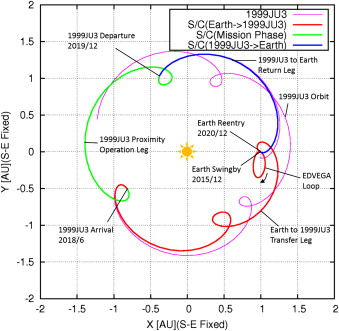
\includegraphics[width=\textwidth]{hayabusa2lowthrust.jpg}
\caption{Trajectory geometry for Hayabusa-2, shown in an inertial reference frame centered at Sun and the line connecting the Sun and Earth is fixed i.e. the Sun-Earth line coincides with the X axis of the inertial frame \cite{ju3lowthrust}.}
\label{fig:hayabusa2transfer}
\end{minipage}
\hspace{0.5cm}
\begin{minipage}[t]{0.45\linewidth}
\centering
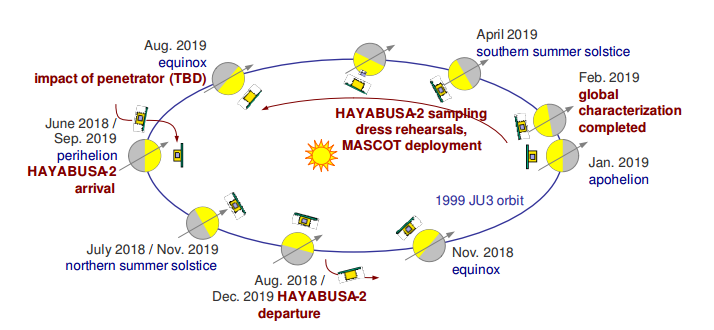
\includegraphics[scale=0.5]{aroundju3traj.png}
\caption{Hayabusa 2 mission phase \cite{ju3traj}.}
\label{fig:aroundju3}
\end{minipage}
\end{figure}


\subsection{Dawn}
\label{dawn}
The Dawn mission of \gls{NASA} was designed to rendezvous and orbit around the asteroids 4 Vesta and 1 Ceres. The objective of the mission was to characterize the asteroids' internal structure, shape, density, size, composition, mass and provide data on surface morphology, cratering, and magnetism \cite{dawnnssdc}.

Vesta and Ceres are two most massive asteroids that have survived largely intact through the collisional history of our solar system. Vesta appears to be a dry and differentiated body consisting of pyroxene-bearing lava flows. Telescopic observations have revealed mineralogical variations along the asteroid's surface. Certain meteorites have been linked to be fragments of Vesta. The latter has a dimension of 289 x 280 x 229 km. Ceres, the largest body in the asteroid belt with a dimension of 487 x 487 x 455 km, is very different from Vesta although its only slightly farther away from Sun than the latter. Microwave observations reveal that Ceres is covered in a clay like material, indicating the presence of water in its history. No meteorites have been linked to Ceres. Vesta, which is believed to be dry and differentiated, and Ceres, which consists of water ice that slowed its thermal evolution, form the bridge between the rocky bodies in the inner solar system and icy bodies in the outer solar system \cite{dawnelsevier}.

The dawn spacecraft was launched in September 2007 on-board a Delta-2 heavy rocket and after an initial checkout phase \cite{vestaorbits}, it was put into its interplanetary orbit towards Vesta. The entire interplanetary trajectory is depicted in \Cref{fig:dawninterplanetary}. The interplanetary cruise was performed using the on-board ion propulsion system. The cruise phase consisted of varying thrusting and strategically designed coasting periods. The latter was included for the ground control to perform orbit determination, downloading spacecraft engineering data and for uploading command sequences to the spacecraft using \gls{NASA}'s \gls{DSN} \cite{dawninter}. After a gravity assist in February 2009, Dawn arrived at Vesta in July 2011 \cite{dawninter}. Four mapping orbits were planned around Vesta at three different mapping altitudes. All the orbits were close to polar inclination. Each orbit started as an instantaneous circular orbit but due to Vesta's gravity, these circular orbits grew into eccentric orbits. The different mapping orbits along with their altitudes are illustrated in \Cref{fig:vestaorbits} \cite{vestaorbits}.

\begin{figure}[h]
\begin{minipage}[t]{0.45\linewidth}
\centering
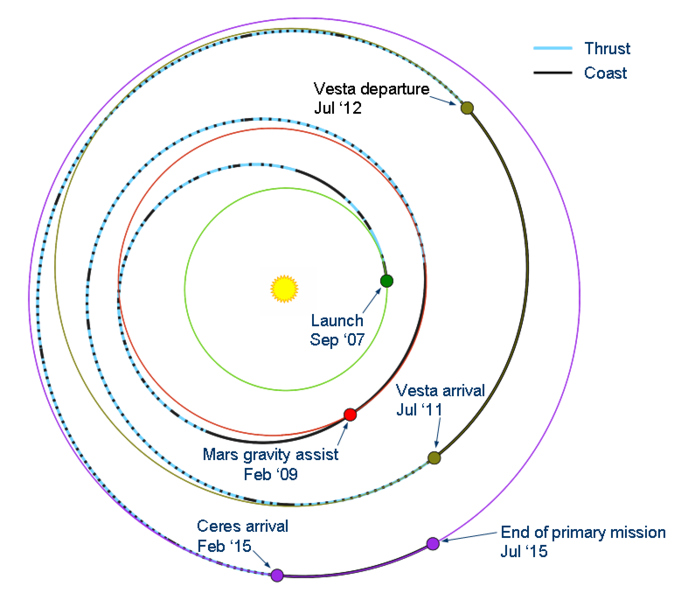
\includegraphics[width=\textwidth]{dawninterplanetary.png}
\caption{Dawn's Interplanetary Trajectory. The trajectory is depicted in blue when thrusting and in black when coasting. \cite{dawninter}}
\label{fig:dawninterplanetary}
\end{minipage}
\hspace{0.5cm}
\begin{minipage}[t]{0.45\linewidth}
\centering
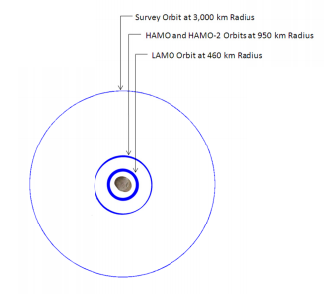
\includegraphics[width=\textwidth]{vestaorbits.png}
\caption{Vesta Science Orbits \cite{vestaorbits}}
\label{fig:vestaorbits}
\end{minipage}
\end{figure}

The first and highest is the survey orbit at an altitude of 3000 km. The angle between Dawn's orbital plane and the Sun-Vesta line keeps increasing as Vesta moves around the Sun. This ensured that Dawn never entered Vesta's shadow in the survey orbit. The next phase is the \gls{HAMO} which lies between the altitudes of 925 and 975 km. The groundtrack of \gls{HAMO} repeated after every 10-orbits. \Cref{fig:vestahamo} illustrates the 10-orbit cycle of \gls{HAMO}. Each equator crossing of the 10-orbit cycle was evenly spaced, around 36 degrees, to get uninterrupted images of Vesta's surface. The angle between the orbital plane and the Vesta-Sun line (henceforth called the $\beta$ angle) was frozen, unlike that of the survey orbit, offering constant illumination of Vesta's surface throughout the mapping process. The third phase was the \gls{LAMO} which lies between the altitudes of 405 and 521 km. \Cref{fig:vestalamo} illustrates the groundtrack of \gls{LAMO}. The groundtrack of \gls{LAMO} ensured total surface coverage in the first 60 days of entering into this orbit by keeping a 6 degree longitudinal spacing between successive equatorial crossings. The $\beta$ angle in \gls{LAMO} was frozen at a target value of 45 degree such that at the given orbital radius, the spacecraft never entered the shadow region (shadow occurred at a $\beta$ angle of 39 degree) \cite{vestaorbits}.

\begin{figure}[h]
\begin{minipage}[t]{0.45\linewidth}
\centering
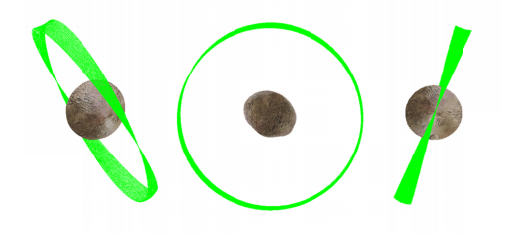
\includegraphics[width=\textwidth]{vestahamo.png}
\caption{10-orbit cycle of \gls{HAMO} design \cite{vestaorbits}.}
\label{fig:vestahamo}
\end{minipage}
\hspace{0.5cm}
\begin{minipage}[t]{0.45\linewidth}
\centering
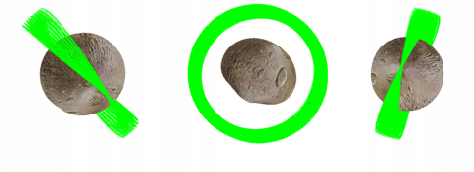
\includegraphics[width=\textwidth]{vestalamo.png}
\caption{Vesta Low-altitude mapping orbit \cite{vestaorbits}.}
\label{fig:vestalamo}
\end{minipage}
\end{figure}

Just like the orbits at Vesta, Dawn had three different types of science orbits at different altitudes around Ceres, see \Cref{fig:ceresorbits}. All of the orbits at Ceres were circular and polar, going from North to South over the side which was illuminated by the Sun. Upon capture at Ceres, Dawn entered into what is known as the \gls{RC3} orbit at an altitude of 13,500 km, see \Cref{fig:rc3}. The \gls{RC3} orbit helped in determining the composition of Ceres along with accurately finding its pole points. The orbital period of \gls{RC3} was 15 days. The orbit geometry was such that the spacecraft always remained in Sunlight, irrespective of the lighting condition on the surface \cite{dawnblog}. In the RC3 orbit, as Ceres completed one full rotation around its own axis (just over 9 hours \cite{dawnblog}), the spacecraft position changed by only about 10 degrees in latitude \cite{ceresorbits}.

\begin{figure}[h]
\begin{minipage}[t]{0.45\linewidth}
\centering
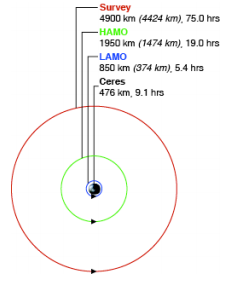
\includegraphics[width=\textwidth]{ceresorbits.png}
\caption{A schematic illustrating the three different orbit phases, their corresponding altitudes and orbital periods around Ceres. The \gls{RC3} orbit is not shown here, which was at an altitude of 13500 km \cite{ceresorbits}.}
\label{fig:ceresorbits}
\end{minipage}
\hspace{0.5cm}
\begin{minipage}[t]{0.45\linewidth}
\centering
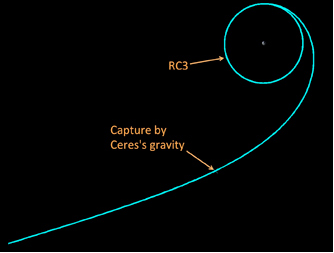
\includegraphics[width=\textwidth]{rc3.png}
\caption{Following capture by Ceres' gravity, Dawn used ion propulsion to spiral down to the \gls{RC3} orbit  \cite{dawnblog}.}
\label{fig:rc3}
\end{minipage}
\end{figure}

After completing its investigations in the \gls{RC3} orbit, Dawn spiraled down to the "survey orbit" which was about 4400 km above the surface of Ceres. During this month-long decent, Dawn made only 5 revolutions around Ceres. \Cref{fig:rc32survey} illustrates the 5 spiral loops that Dawn traversed to reach the survey orbit. After finalizing observations in the survey orbit, Dawn spiraled down in a tighter loop to \gls{HAMO} (at 1470 km) in about 30 revolutions around Ceres in a six week long trip. After performing two months of intense observations in \gls{HAMO}, the spacecraft spiraled down to the final orbit called \gls{LAMO} at 375 km in the most tight loop possible of 160 revolutions around Ceres in just two months of trip time  \cite{dawnblog2}. \Cref{fig:hamo2lamo} illustrates the tight spiraling transfer from \gls{HAMO} to \gls{LAMO}.

\begin{figure}[h]
\begin{minipage}[t]{0.45\linewidth}
\centering
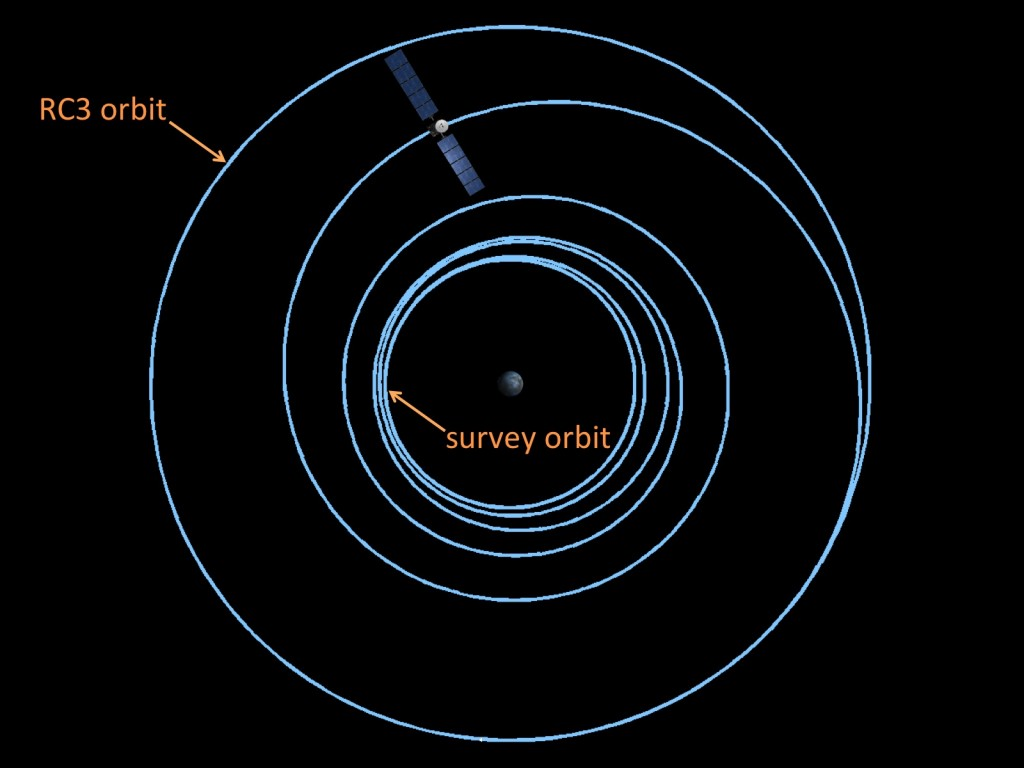
\includegraphics[width=\textwidth]{rc32survey.jpg}
\caption{Spiral loop traversed by Dawn to reach survey orbit from \gls{RC3} \cite{dawnblog2}.}
\label{fig:rc32survey}
\end{minipage}
\hspace{0.5cm}
\begin{minipage}[t]{0.45\linewidth}
\centering
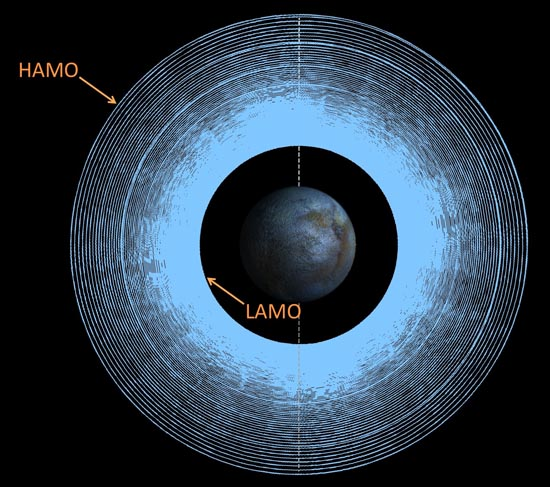
\includegraphics[width=\textwidth]{hamo2lamo.jpg}
\caption{Tight spiral traversed by Dawn from \gls{HAMO} to \gls{LAMO} in 160 revolutions around Ceres \cite{dawnblog2}.}
\label{fig:hamo2lamo}
\end{minipage}
\end{figure}

Each revolution in the survey orbit was defined as a mapping cycle and each cycle was planned to cover different regions of Ceres. The 7 revolutions in the survey orbit achieved 95$\%$ surface coverage of Ceres \cite{ceresorbits}. \Cref{fig:surveyatceres} shows the surface regions covered by different revolutions (or mapping cycles) in the survey orbit around Ceres. At the \gls{HAMO} altitude, the spacecraft had an orbital period of 19 hours. \gls{HAMO} consisted of five mapping cycles and each cycle consisted of 14 orbits and at the designated altitude for \gls{HAMO}, only 12 orbits were required to give a complete coverage of the surface \cite{ceresorbits}. The ground coverage by Dawn in \gls{HAMO} is illustrated in \Cref{fig:hamoatceres}.

\begin{figure}[h]
\begin{minipage}[t]{0.45\linewidth}
\centering
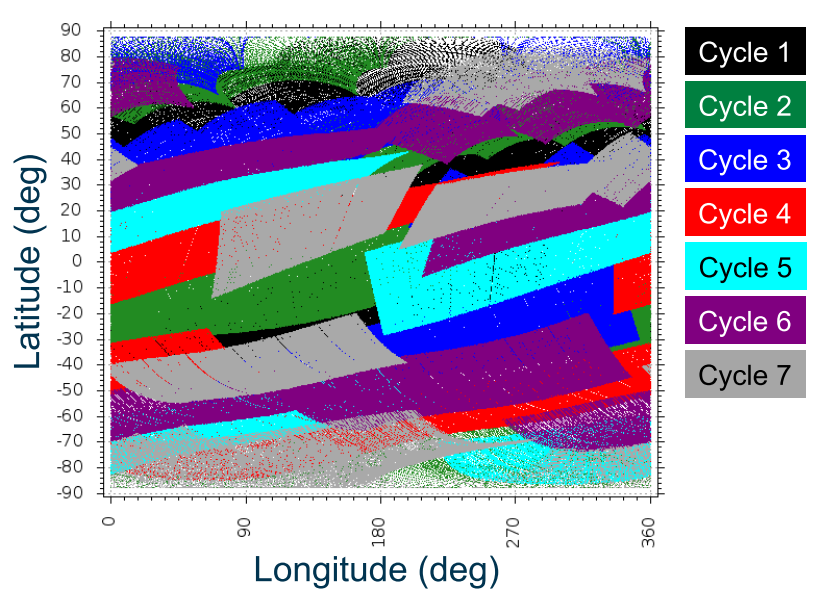
\includegraphics[width=\textwidth]{surveyatceres.png}
\caption{Ground coverage by Dawn in multiple revolutions (cycles) in the survey orbit around Ceres. Each cycle was planned to cover a different region of Ceres' surface which resulted in an irregular patchwork of observation. The overlaps in the observation between different cycles provided redundancy against data loss \cite{ceresorbits}.}
\label{fig:surveyatceres}
\end{minipage}
\hspace{0.5cm}
\begin{minipage}[t]{0.45\linewidth}
\centering
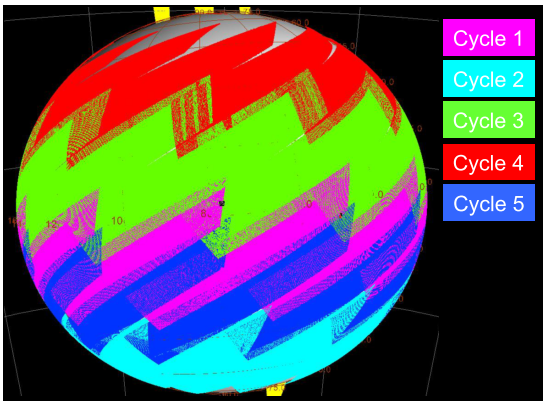
\includegraphics[width=\textwidth]{hamoatceres.png}
\caption{Ground coverage by Dawn in \gls{HAMO} around Ceres. Each cycle consisted of 14 orbits and each orbit had a period twice that of the rotation period of Ceres. Each cycle was planned to cover a different latitude band \cite{ceresorbits}.}
\label{fig:hamoatceres}
\end{minipage}
\end{figure}

Following the departure from \gls{HAMO}, the spacecraft arrived at the altitude of 375 km of the \gls{LAMO}, with an orbital period of 5.4 hours. The total revolutions in \gls{LAMO} were divided into four cycles each with 101 orbital revolutions. Each cycle of 101 orbits was comprised of five repeating 20 orbit segments (plus one phasing orbit). The \gls{LAMO} altitude selection was a major challenge for the Dawn team since hydrazine consumption (hydrazine is used on-board Dawn by the \gls{RCS} for attitude control) increased for altitudes below 1000 km. Apart from selecting the proper altitude, the orbit designers for \gls{LAMO} had to ensure that the orbit can also provide dense ground coverage to meet the science objectives \cite{ceresorbits}.

\subsection{Rosetta}
\label{rosetta}
Rosetta is a cornerstone mission of \gls{ESA}'s scientific program. The prime objective of the Rosetta comet rendezvous mission was in-situ observations of cometary matter. The original mission was supposed to be launched in July 2003 and reach comet Wirtanen in 2011 \cite{rosettaoldmartin}. However, Rosetta lost its 19 day launch window in 2003 due to suspension of Ariane 5 launches following the failure of flight 517 in 2002. A new mission opportunity was selected, soon after loosing the first launch window, which was subsequently launched in 2004 and rendezvoused with comet 67P/Churyumov-Gerasimenko (henceforth called 67P/CG) in 2014 \cite{rosettanewferri}.

\subsubsection{Orbit around comet Wirtanen}
In case of a comet, orbit strategies cannot be fixed beforehand and are to be decided during the late comet approach phase. This is so because comet properties cannot be completely determined from Earth-based (ground and/or satellite) observations due to large distances of cometary orbit from Earth. Although Rosetta never flew to the comet Wirtanen, the following description briefly describes the preliminary orbit design for the spacecraft around the comet \cite{rosettaoldmartin}.

The sphere of influence in which the gravitational attraction of the Sun can be considered as a perturbation, given that only Earth-observed mean comet nucleus radius and density information is available, will have a size ranging from 7 to 20 times the cometary nucleus radius. Orbits near the comet can be considered as Keplerian orbits i.e. at altitudes of a few cometary radii, since the effect of a non-spherical gravity field will have minor influence on the motion of the spacecraft. Mapping of the comet would have been done with eccentric orbits around it, wherein the orbital plane would have been such that it contained the comet's spin axis and the comet-Sun line. The close observations phase was planned to consist of a sequence of eccentric orbits, all at altitudes of or below 1 cometary nucleus radius. To deliver the surface probe, the spacecraft was planned to be transferred into an elliptic orbit around the comet so that the orbiter could fly multiple revolutions without any maneuvers and obtain precise knowledge on the orbit of the spacecraft, thus ultimately leading to a good probe delivery accuracy. Following the delivery of the surface probe, the orbiter was planned to enter a relay orbit to communicate with the ground stations on Earth. \Cref{fig:rosettaoldmartin} illustrates the geometries of the different types of orbits around comet Wirtanen \cite{rosettaoldmartin}.

\begin{figure}[htb]
\begin{minipage}[t]{0.45\linewidth}
\centering
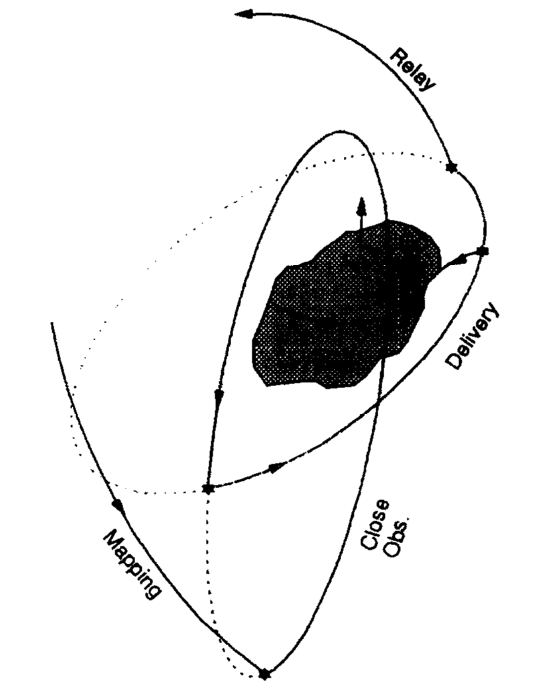
\includegraphics[width=\textwidth]{rosettaoldmartin.png}
\caption{Rosetta orbits around comet Wirtanen \cite{rosettaoldmartin}.}
\label{fig:rosettaoldmartin}
\end{minipage}
\hspace{0.5cm}
\begin{minipage}[t]{0.45\linewidth}
\centering
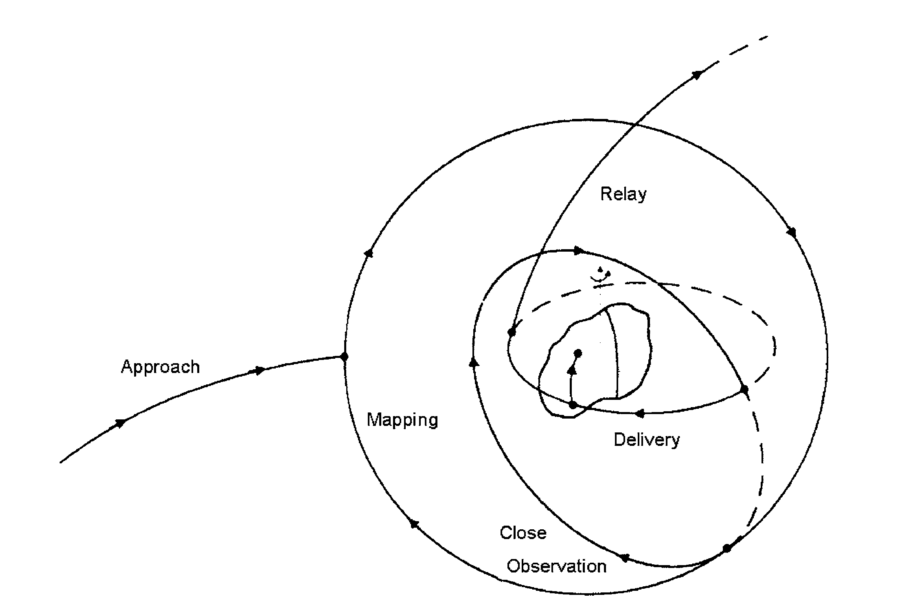
\includegraphics[width=\textwidth]{rosettanew2007.png}
\caption{Schematic of Rosetta's different orbits around 67P/Churyumov-Gerasimenko \cite{rosettanew2007}. Note the similarity with the preliminary orbit design of Rosetta around comet Wirtanen, depicted in \Cref{fig:rosettaoldmartin}.}
\label{fig:rosettanew2007}
\end{minipage}
\end{figure}

\subsubsection{Orbit around comet 67P/Churyumov-Gerasimenko}
We will now discuss the orbit design around the new target comet, 67P/CG. The initial orbit design, before complete cometary information of 67P/CG was known, is illustrated in \Cref{fig:rosettanew2007}. At a distance of 300 times the cometary nucleus radius, the relative velocity between the spacecraft and the comet was reduced to about 1.5 m/s. At this point, landmark and radiometric measurements were performed for precise determination of the relative position and velocity of Rosetta and 67P/CG, and the gravity and rotation of the comet. The new in-situ information was then used to start the orbit insertion around the comet and initiate close proximity operations at a distance of about 60 times the cometary nucleus radius, with a relative velocity of just a few cm/s. At a distance of 25 times the cometary nucleus radius, the spacecraft was captured into a closed orbit around the comet. For global mapping of the cometary nucleus, polar orbits with altitudes ranging from 5 to 25 times the cometary nucleus radius were used. After concluding global observations, close proximity operations around the comet began in orbits with altitudes of 1 cometary nucleus radius. Based on the data collected in close proximity observations, the landing site for the Philae lander was selected. The lander was deployed from an eccentric orbit with pericenter altitude being very close to the landing site \cite{rosettanew2007}. After deploying the lander, Rosetta was transferred into an orbit suitable for transmitting data back to Earth, see \Cref{fig:rosettanew2007}. Now, we shall discuss the different orbits around the comet in more detail.

\textbf{Comet Initial Characterization Phase:} The objective of this phase, was for the spacecraft to fly around the comet and identify landmarks on the comet's surface, estimate its shape and rotation state and get an initial estimation of its gravitational field. This information was used to fly trajectories much closer to the surface, in the subsequent phase. The trajectory in the initial characterization phase consisted of 4 hyperbolic arcs in the shape of a pyramid, see \Cref{fig:rosettainitchartraj}, on the day side of the comet. The first arc started at a 100 km distance, while every other arc had a pericenter distance of about 60 km. Each arc lasted for 2 days. Each orbital plane, corresponding to each of the arcs, was tilted at an angle of 45 degrees from the Sun's direction. An impulse of 0.7 m/s was required to switch between the arcs. The reason why hyperbolic arcs were selected instead of circular/elliptical ones, was that hyperbolic trajectories result in higher relative velocity between the spacecraft and the comet, which makes the trajectory more robust against insertion maneuver errors and the mis-modeling of spacecraft dynamics around the comet. Also, with faster arcs, the comet can be observed in shorter time \cite{rosettanew2012}.

\begin{figure}[h]
\centering
\captionsetup{justification=centering}
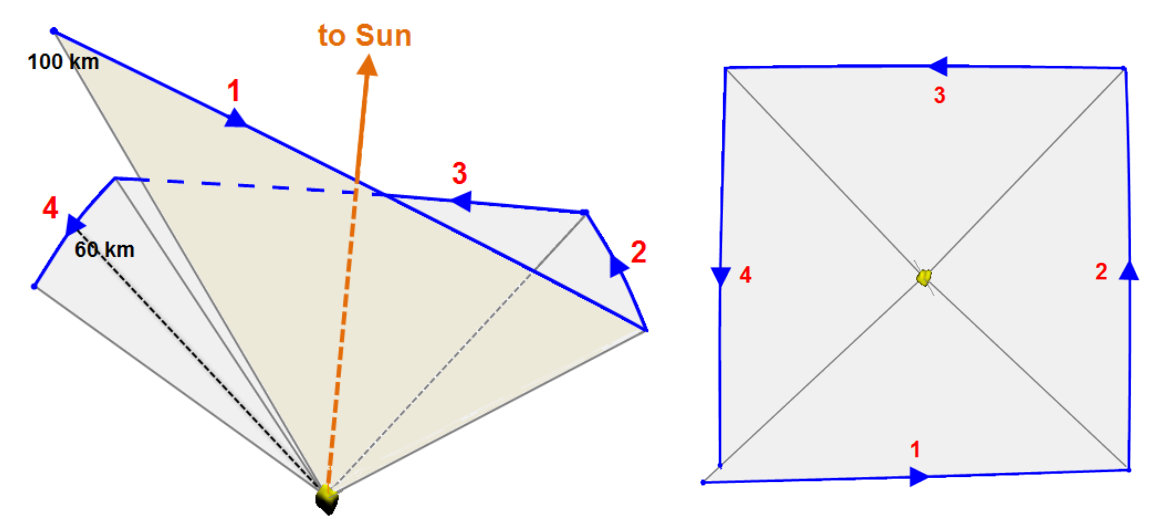
\includegraphics[scale=0.4]{rosettainitchartraj.png}
\caption{Geometry of Rosetta's initial characterization phase around 67P/CG \cite{rosettanew2012}.}
\label{fig:rosettainitchartraj}
\end{figure}

\textbf{Global Mapping Phase:} This phase was planned to improve upon the knowledge on dynamical properties and kinematics of the comet. The selected trajectory, see \Cref{fig:rosettaglobalmappingtraj}, consists of four 180-degree arcs of circular polar orbit, each having a radius of 20 km. These arcs are found in two orbital planes each having a 30 degree inclination from the Sun direction, to avoid eclipses. To keep the spacecraft on the day-side of the comet, the transfer maneuver from one arc to the other were performed when the spacecraft was above the poles of the comet. By skipping one maneuver (i.e. instead of a 180 degree arc, the spacecraft completes the whole 360 degree orbit), in either plane, a night-side excursion of the comet is also possible. Each maneuver to shift between the arcs also changes the orbital plane from morning to afternoon and vice-versa \cite{rosettanew2012}, see \Cref{fig:rosettaglobalmappingtraj}.

\begin{figure}[h]
\centering
\captionsetup{justification=centering}
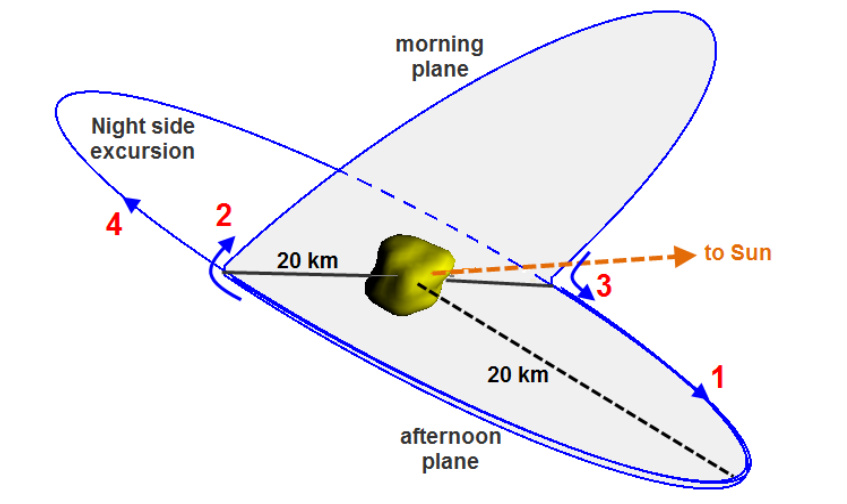
\includegraphics[scale=0.5]{rosettaglobalmappingtraj.png}
\caption{Geometry of Rosetta's global mapping phase around 67P/CG \cite{rosettanew2012}.}
\label{fig:rosettaglobalmappingtraj}
\end{figure}

\textbf{Close Observation Phase:} This phase was used to select candidate landing sites (for the Philae lander) based on the information obtained in the previous phase. Accurate information on spacecraft navigation was required to allow the instruments to point towards the candidate landing sites. This information was obtained by executing a trajectory around the comet without any impulsive maneuvers because any uncertainty in maneuver performance would have lead to degradation of navigation knowledge around the comet. One of the mission requirements was to have continuous optical observations of the comet and hence any trajectory to the night-side of the comet was avoided. The candidate landing sites were observed from a circular orbit of 10 km radius lying in the daylight terminator plane around the comet to avoid night-side excursions. A terminator plane is one where the spacecraft flies above the day-night line, in this case, on the comet's surface. After determination of one of the candidate landing sites, an orbit closer to the surface was selected to observe the landing site at the pericentre passage. This orbit was elliptical with the apocentre at 10 km radius and pericentre at 5 km radius \cite{rosettanew2012}. \Cref{fig:rosettacloseobstraj} illustrates the orbits of the close observation phase. The reader is advised to scan the QR code given in \Cref{fig:QR1} to view the trajectory animation by \gls{ESA} for the initial characterization, global mapping, and the close observation phases.

\textbf{Lander Delivery Phase:} In this phase, Rosetta entered into a trajectory from which the lander was deployed towards the comets' surface. The spacecraft was initially in an orbit similar to the one in the close observation phase. It was maneuvered and put into a hyperbolic trajectory and soon after the lander was separated \cite{rosettanew2012}. \Cref{fig:rosettalandertraj} illustrates the geometry of the trajectory and the lander separation point. The reader is also advised to scan the QR code given in \Cref{fig:philaedeliveryQR} to view the trajectory animation by \gls{ESA} for the lander delivery phase.

\begin{figure}[h]
%\begin{minipage}[t]{0.45\linewidth}
\centering
\captionsetup{justification=centering}
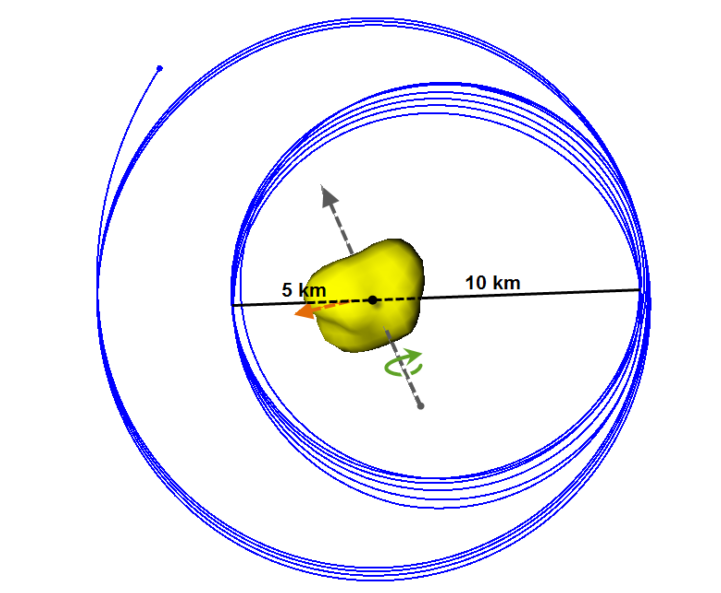
\includegraphics[scale=0.5]{rosettacloseobstraj.png}
\caption{Geometry of Rosetta's close observation phase around 67P/CG \cite{rosettanew2012}.}
\label{fig:rosettacloseobstraj}
\end{figure}

\begin{figure}[htb]
\begin{minipage}[t]{0.45\linewidth}
\centering

\includegraphics[scale=0.5]{rosettatriangularorbitQR.png}
\caption{Animation by \gls{ESA} depicting Initial characterization, global mapping and close observation phases. Scan the QR code to view the trajectory animation or visit the following web-link: \url{https://www.youtube.com/watch?v=fNBUep7mPdI&feature=youtu.be}}
\label{fig:QR1}
\end{minipage}
\hspace{0.5cm}
\begin{minipage}[t]{0.45\linewidth}
\centering

\includegraphics[scale=0.5]{philaedeliveryQR.png}
\caption{Animation by \gls{ESA} depicting lander delivery phase of Rosetta. Scan the QR code to view the trajectory animation or visit the following web-link: \url{https://www.youtube.com/watch?v=4a3eY5siRRk&feature=youtu.be}}
\label{fig:philaedeliveryQR}
\end{minipage}
\end{figure}
\FloatBarrier

\begin{figure}[h]
%\begin{minipage}[t]{0.45\linewidth}
\centering
\captionsetup{justification=centering}
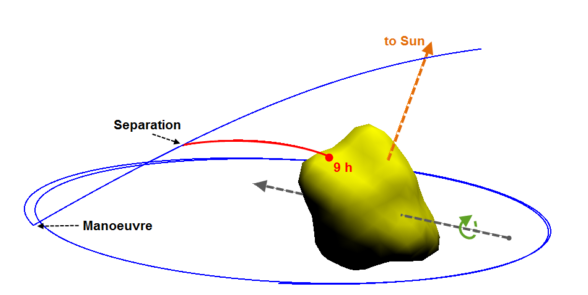
\includegraphics[scale=0.9]{rosettalandertraj.png}
\caption{Geometry of Rosetta's lander delivery phase to 67P/CG \cite{rosettanew2012}.}
\label{fig:rosettalandertraj}
\end{figure}

\subsection{NEAR}
\label{Near}
The \gls{NEAR} mission was designed to study the near-Earth Asteroid Eros from a close orbit over a period of one year. The \gls{NEAR} spacecraft was launched in 1996, and with an Earth swingby in January 1998, the spacecraft was targeted towards Eros. However due to a main engine abort in December 1998, a fly-by of Eros was performed and a rendezvous was rescheduled for the year 2000 \cite{erosbook}.

\begin{figure}[h]
\centering
\captionsetup{justification=centering}
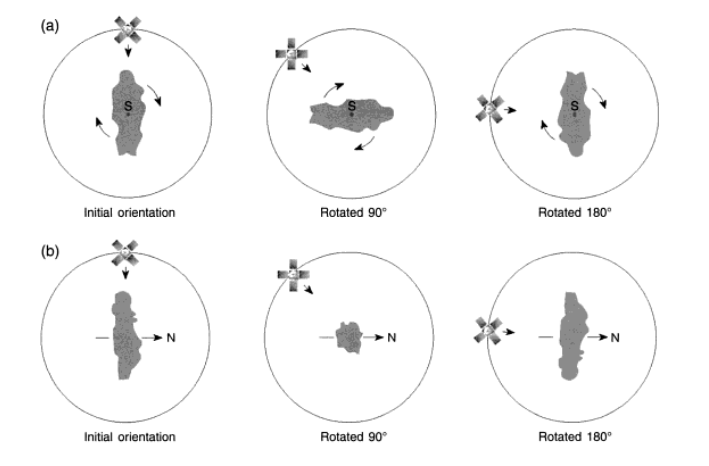
\includegraphics[scale=0.6]{nearerosbook.png}
\caption{Orbital geometries around Eros, as viewed from the Sun. The arrow near the spacecraft marks the instrument bore-sight. (a) Spacecraft is in a retrograde equatorial orbit and the south pole of Eros is denoted by 'S'. (b) Spacecraft is in a polar orbit and the arrow going through the asteroid denotes its spin axis \cite{erosbook}.}
\label{fig:nearerosbook}
\end{figure}

\Cref{fig:nearerosbook} illustrates a schematic of the geometry of the low-altitude circular orbit around Eros as viewed from the Sun. The orbital plane is always within 30 degrees of a plane which is perpendicular to the Eros-Sun line, so as to orient the spacecraft's fixed solar panel towards the Sun. In part (a) of \Cref{fig:nearerosbook}, the spacecraft is in a circular equatorial orbit with its spin axis aligned with the Eros-Sun line. The south pole of Eros is facing the Sun and the spacecraft orbit is retrograde. Part (b) of \Cref{fig:nearerosbook} denotes the earlier part of the orbital mission wherein the asteroid rotation axis was perpendicular to the Eros-Sun line and the spacecraft orbit was in a polar orbit \cite{erosbook}.

\begin{figure}[h]
\centering
\captionsetup{justification=centering}
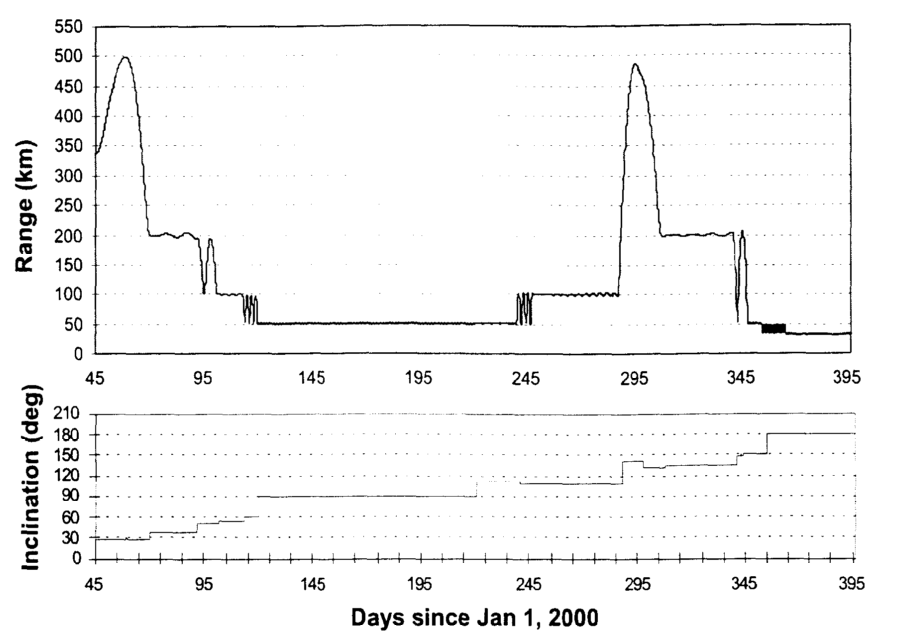
\includegraphics[scale=0.35]{erosprofile.png}
\caption{Range and Inclination in orbit phase around Eros \cite{erosprofile}.}
\label{fig:erosprofile}
\end{figure}

\Cref{fig:erosprofile} shows the mission profile of the \gls{NEAR} spacecraft in terms of its distance from the asteroid and inclination of its orbital plane from the asteroid's equator while it was in a close circular orbit. The long duration of \gls{NEAR} in a polar orbit at a range of 50 km was designed to permit the most comprehensive mapping of Eros. The low-altitude retrograde orbit towards the end of mission profile was designed to extensively map the equatorial region of Eros \cite{erosprofile}.

The methodology adopted for orbit design of the \gls{NEAR} mission was to compute a maneuver that satisfied a local set of constraints and performance criteria and then propagate the trajectory to see where it goes. This differs substantially from the traditional approach of defining a number of constraints and then obtaining a trajectory that is a global minimum of some performance criteria \cite{erosapproach}. From the orbit design approach adopted by the \gls{NEAR} mission designers, it can be inferred that their approach allows a relatively simple way to compute trajectories, because instead of solving for global constraints that are defined for all the scientific objectives, they solved for orbits under local constraints pertaining to fewer or even singular scientific objectives at a time and then repeated this step-by-step process until all scientific objectives were met. Although this approach will provide locally optimum trajectories, it is not necessary that these trajectories would also be globally optimum.

\section{Future Missions}
\label{future}
% Talk about ESA's AIM and NASA's asteroid redirect mission here. (look into dan's book for this also). Search for Jaxa's future missions as well. Also about the private venture DSI's goal of minig asteroids
This section will discuss the missions proposed or planned for the future.

\subsection{OSIRIS-REx}
\label{osiris-rex}
In September 2016, the \gls{OSIRIS-REx} spacecraft will be launched to rendezvous with asteroid Bennu. After arriving at the asteroid in 2018, it will conduct observations to select a suitable site from where it will retrieve a sample of the asteroid and return it to Earth in 2023 \cite{osiris}.

The mission design of \gls{OSIRIS-REx} consists of a preliminary survey phase that comprises of three hyperbolic passes over the North and South poles and the equator at a distance of 7 km from the centre of the asteroid, see \Cref{fig:osirishyper}. These passes will determine information about the asteroid which will be necessary in planning the propulsive maneuvers to place the spacecraft in an orbit around it \cite{osiris}.

After the preliminary survey phase, the spacecraft will enter into an orbit at a distance of 1.5 km (Orbital A) from the centre of the asteroid. In Orbital A, the spacecraft will transition to landmark based optical navigation. The spacecraft will also perform high resolution science imaging during Orbital A phase to improve topographic maps and shall also determine the rotation state of the asteroid \cite{osiris}.

Following the Orbital A phase, comes the final leg in the global investigation of Bennu, the detailed survey phase consisting of multiple hyperbolic passes of Bennu. The first of these passes will be at a distance of 3.5 km from the centre of the asteroid and transit over four sub-satellite points at 40 degrees latitude (both North and South) and at 10 AM and 2 PM local time at the surface of Bennu. Following this, the spacecraft will traverse in seven passes at an altitude of 5 km from the surface of the asteroid. These passes fly through points above the equator spaced over multiple local times of day on the surface, see \Cref{fig:osirisorbits}. The end of the detailed survey phase will result in an initial selection of 12 candidate sites from where a sample of the asteroid could potentially be collected \cite{osiris}.

\begin{figure}[h]
\begin{minipage}[t]{0.45\linewidth}
\centering
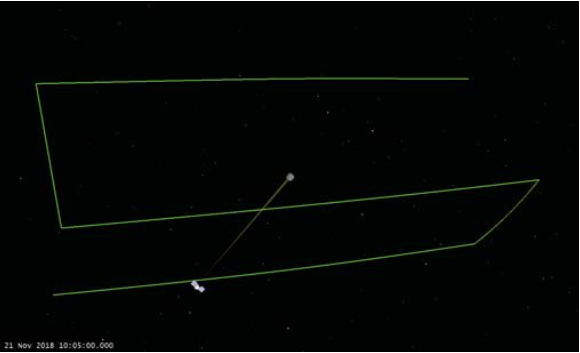
\includegraphics[width=\textwidth]{osirishyper.png}
\caption{Hyperbolic passes over both the poles and the equator, as part of the preliminary survey of asteroid Bennu \cite{osiris}.}
\label{fig:osirishyper}
\end{minipage}
\hspace{0.5cm}
\begin{minipage}[t]{0.45\linewidth}
\centering
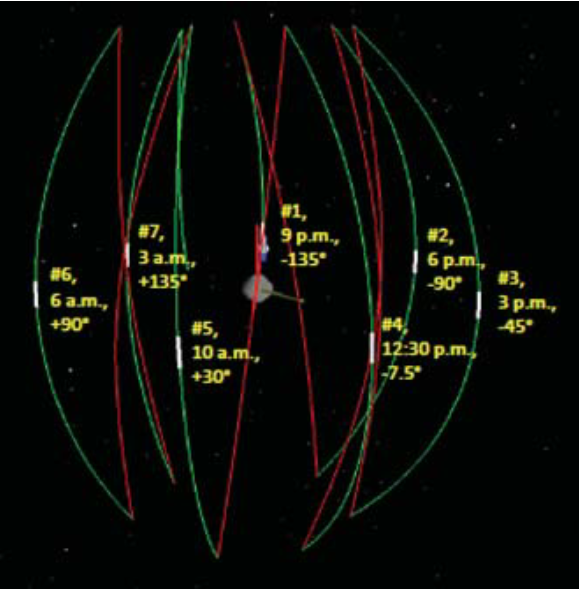
\includegraphics[width=\textwidth]{osirisorbits.png}
\caption{Multiple passes through points above the equator of Bennu, as part of the detailed survey of the asteroid \cite{osiris}.}
\label{fig:osirisorbits}
\end{minipage}
\end{figure}
\FloatBarrier

Following the Detailed Survey phase, the spacecraft will perform a site-specific reconnaissance mission on the initial selection of candidate sampling sites. To do this the spacecraft will enter into a 1 km orbit (Orbital B) around Bennu. This phase will conclude with the selection of two primary and two secondary sites. The two primary sites will be observed again from an altitude of 225 m above the surface of the asteroid to get high-resolution images of the surface \cite{osiris}.

\subsection{AIDA}
\label{aida}
The \gls{AIDA} mission will be the first of its kind to demonstrate a mitigation technique to protect Earth from an asteroid impact by performing a spacecraft kinetic impact on the asteroid to deflect it from its trajectory. \gls{AIDA} is an international collaboration between \gls{ESA} and \gls{NASA}. Both space agencies will provide independent but mutually supporting missions. \gls{NASA} will provide the asteroid kinetic impactor spacecraft under its \gls{DART} mission and \gls{ESA} will provide the asteroid characterization spacecraft under its \gls{AIM}. The \gls{AIDA} target will be the binary asteroid Didymos and the deflection experiment will take place in late 2022 \cite{aida}. \Cref{fig:aim} shows the heliocentric trajectory of Didymos along with that of Earth and other inner solar system planets.

Since this literature survey report is focused on the design of orbits around asteroids, hence this subsection shall present information on the \gls{AIM} part of the \gls{AIDA} mission. \gls{AIM} shall start the observation of the Didymos binary system from a formation-flying quasi periodic orbit at an altitude of 35 km which is outside the sphere of influence of both asteroids in the Didymos system. This station point will be within the orbital plane of the asteroid around the Sun but it will be offset by around 45 degrees from the direction towards the Sun. This ensures that the spacecraft will always be positioned above the illuminated face of the asteroid. To perform a more detailed characterization of the asteroid, a second observation station point is selected at a 10 km altitude. Finally, as part of the \gls{AIDA} mission scenario, the \gls{DART} impactor will be observed from a safe distance of 100 km from Didymos to avoid any damage from the impact debris \cite{aida}.

\begin{figure}[h]
\centering
\captionsetup{justification=centering}
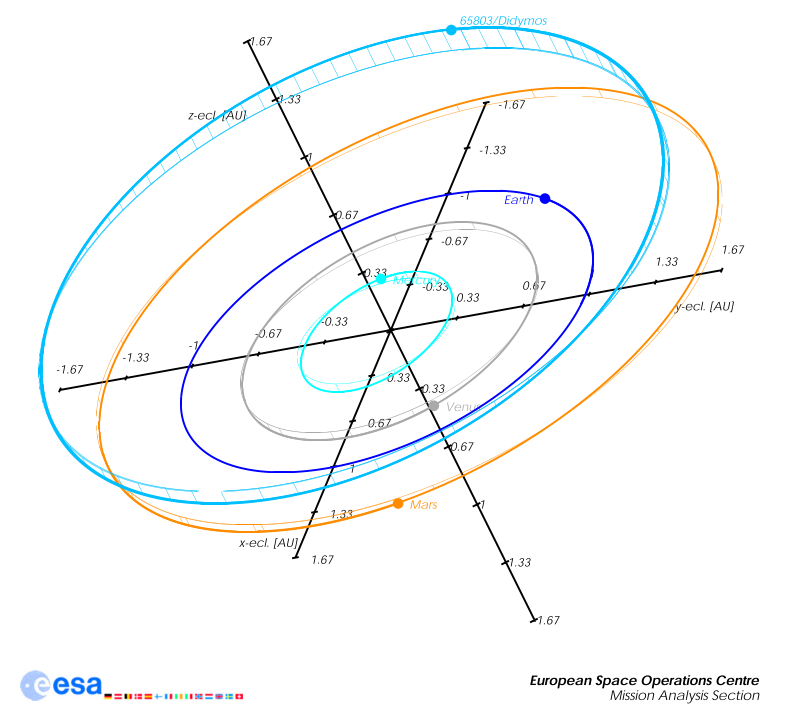
\includegraphics[scale=0.5]{aim.png}
\caption{Heliocentric orbit of the Didymos system \cite{aida}.}
\label{fig:aim}
\end{figure}
\FloatBarrier

\section{Conclusion}
\label{heritage_conclusion}
In this chapter we discussed a few missions to asteroids that were conducted in the past, some which are being conducted presently, and some that will be conducted in the future. The idea behind writing this chapter, was to understand the approach that has been adopted for different mission scenarios, to gather any common elements, and to understand the reasons behind following a particular approach to orbit design. The inferences drawn from studying the various missions are listed as follows:
\begin{itemize}
\item The design of all propulsive maneuvers and all the trajectories in between those maneuvers, are always driven by the scientific objectives and spacecraft constraints, not the other way around.
\item Since the dynamical environment around small bodies such as asteroids and comets is not always known to a very high accuracy, due to the inability to perform the required observations at such large distances from Earth, a common approach to orbit design involves breaking down the mission into multiple phases in terms of the altitudes of the orbits around the small body. For example, before planning maneuvers and designing orbits for close proximity operations, the spacecraft would first map the rotation rates, composition, and gravitational attraction of the small body from a relatively large distance in what is usually defined as a survey orbit, and then proceed to lower altitudes gradually to perform the scientific objectives.
\item Due to relatively low gravitational attraction of asteroids and comets, it is always possible to design trajectories around the small body which involves multiple propulsive maneuvers since the cost of these maneuvers is small.
\end{itemize}
